\documentclass[12pt,a4paper,english]{article}
\usepackage[english]{babel}
\usepackage[utf8]{inputenc}
\usepackage{svg}
\usepackage{amsmath}
\usepackage{johd}
%\usepackage{natbib}
\usepackage{numprint}
\usepackage{dcolumn}
\newcolumntype{d}[1]{D{.}{.}{#1}}
\usepackage{siunitx}
\newcommand{\round}[2]{\num[round-mode=places,round-precision=#1]{#2}}
\usepackage{booktabs}
\usepackage{authblk}
\usepackage{hyperref}
\hypersetup{
    colorlinks=true,
    linkcolor=blue,
    filecolor=blue,      
    urlcolor=blue,
}
\usepackage[backend=biber, style=bwl-FU]{biblatex}
\addbibresource{bibliography.bib}
\npdecimalsign{.}
\nprounddigits{2}
\title{Stock Market Capitalization vs. GDP Growth}
\author[1]{Martina Stieger}
\author[1]{Flurina Schneider}
%\affil{University of Zurich, Plattenstrasse 14, 8032 Zurich, Switzerland
\author[1]{Till Furger}
\author[1]{Luis Onesimo Leonardo Escobar Farfan}
\affil[1]{University of Zurich, Plattenstrasse 14, 8032 Zurich, Switzerland}

    
%\author{
%    
%    Martina Stieger\thanks{University of Zurich, Plattenstrasse 14, 8032 Zurich, Switzerland, \tt{martina.stieger@uzh.ch}} \rule{0.5in}{0pt}
%
 %   Flurina Schneider\thanks{University of Zurich, Plattenstrasse 14, 8032 Zurich, Switzerland, \tt{flurina.schneider@uzh.ch}} \rule{0.5in}{0pt}
%        
%    Luis Escobar\thanks{University of Zurich, Plattenstrasse 14, 8032 Zurich, Switzerland, \tt{luis.escobar@uzh.ch}} \rule{0.5in}{0pt}
%    
 %   Till Furger\thanks{Department of Business Administration and Wineus AG, University of Zurich, Plattenstrasse 14, 8032 Zurich, Switzerland, \tt{till.furger@uzh.ch}}\\
%    
%    \small \date{\today}
%}


\begin{document}


%%%%%%%%%%%%%%%%%%%%%%%%%%%%%%%%%%%%%%%%%%%%%%%%%%%%%%%%%%%%%%%%%%%%%%%%%%%%%%%%%%%%%%%%%%%%%%%%%%%%%%%%%%
% TITLE PAGE %%%%%%%%%%%%%%%%%%%%%%%%%%%%%%%%%%%%%%%%%%%%%%%%%%%%%%%%%%%%%%%%%%%%%%%%%%%%%%%%%%%%%%%%%%%%%
%%%%%%%%%%%%%%%%%%%%%%%%%%%%%%%%%%%%%%%%%%%%%%%%%%%%%%%%%%%%%%%%%%%%%%%%%%%%%%%%%%%%%%%%%%%%%%%%%%%%%%%%%%

\maketitle

\begin{abstract} 
\noindent In order to show our programming skills learned in the course "Digital Tools for Finance" we are
	handing in a short paper, describing the relationship of the growth of gross domestic product (GDP) and stock
	market growth, with a focus on the situation in the United States from 2000 to 2022. We find that over the observed time period, the stock market grew almost seven times more than the national GDP. We compare our result to the growth rates from Indonesia and Mexico from January 2000 to the third quarter of 2022, the latest available value in the data sources. The growth of the stock market is even higher for Indonesia and Mexico. Both Indonesia's mean stock index growth rate and GDP growth rate exceed the respective ones of the United States. Mexico's mean GDP growth rate is below the US mean growth GDP rate, while its mean stock index growth rate above the one of the US. If we interpret the results according to the Buffet Indicator, there might be a potential for a bubble. 
\end{abstract}

\hfill

\noindent\jel{G1, G12}\\
\noindent\keywords{GDP; Growth; Stock Market}\\

\newpage

%%%%%%%%%%%%%%%%%%%%%%%%%%%%%%%%%%%%%%%%%%%%%%%%%%%%%%%%%%%%%%%%%%%%%%%%%%%%%%%%%%%%%%%%%%%%%%%%%%%%%%%%%%
% BEGINNING OF PAPER %%%%%%%%%%%%%%%%%%%%%%%%%%%%%%%%%%%%%%%%%%%%%%%%%%%%%%%%%%%%%%%%%%%%%%%%%%%%%%%%%%%%%%%%%
%%%%%%%%%%%%%%%%%%%%%%%%%%%%%%%%%%%%%%%%%%%%%%%%%%%%%%%%%%%%%%%%%%%%%%%%%%%%%%%%%%%%%%%%%%%%%%%%%%%%%%%%%%

\tableofcontents
\listoffigures
\listoftables
\newpage
\section{Introduction}
\noindent In this project, we are examining whether the stock market capitalization grows faster than the GDP, with a focus on developed countries, namely the United States in the years from 2000 to 2022. The ratio between a country's market capitalization and its GDP is also called the ``Buffet indicator'' and is often used to gain insights about under- or overvaluation of the stock market. We find that over the time period observed, the stock market (SP500) grew almost seven times more than the national GDP. We are comparing the results to the situation in Indonesia and Mexico in order to bring forth similarities and differences between the situation in high income and middle income countries. For these countries, we use data from January 2000 to the third quarter of 2022, the latest available value in the data sources. According to the World Bank, Indonesia is a lower middle income country, and Mexico is an upper middle one. Both countries have a similar macroeconomic behaviour, however, they are representative of two different regions, namely, East-Asia \& Pacific, and Latin America \& Caribbean.


%\newline
\indent In order to visualize these deviations effectively, we have developed an \href{https://flurinaschneider.shinyapps.io/DTFF22/}{interactive app in R Shiny} where each user can undertake robustness checks on his own. We have considered visualisation principles for our graphs and apps and designed them in a colorblind-friendly manner. Finally, we also compare our research to the findings of selected studies and papers in the field.
\newline
Comparing stock market growth to GDP growth can give an indication about the health of an economy and shows the performance of different companies relative to the value of goods and services produced in the economy. If the stock market grows at a faster rate, a potential explanation can be that corporations are outperforming the broader economy, for example because they are in a privileged position or are benefiting from certain positive economic or political conditions. Current research mainly focuses on comparing corporate earnings to the gross domestic products. Other papers investigate the market capitalization and the GDP in absolute terms, without focusing on their growth rate. Additionally, current research usually focuses on only developed or emerging countries, respectively. Or they look into a specific region only, such as Latin American or European countries.
Our research on the other hand undertakes cross-comparisons between high income and middle income country across geographies: We examine three different countries across the globe, which are at three different development stages. 

\section{Literature Review}

According to \cite{investo_stock_gdp}, a rise in equity markets can affect the GDP by influencing financial conditions as well as consumer confidence and behavior. If share prices fall, it can impact investor sentiment adversely and shareholders sell their stock in order to prevent losses, and consumer spending decreases. On the other hand, if the GDP rises, corporate earnings usually increase and investors are bullish for stocks. %https://www.investopedia.com/ask/answers/033015/how-does-stock-market-affect-gross-domestic-product-gdp.asp

\cite{barra_is_2010} examine the growth of GDP and aggregate corporate earnings, considering data ranging from the year 1929 to 1980. They conclude that the growth in the gross domestic product and the aggregate corporate earnings have been similar throughout the last 80 years, except for 1932 and 1933. In said period, the profits were negative. They conclude that their findings favor supply-side models, meaning that in the long-term, corporate earnings in the aggregate and the GDP have the tendency to grow at the same rate. 
%https://www.msci.com/documents/10199/a134c5d5-dca0-420d-875d-06adb948f578

\cite{kuvshinov_big_2022} investigate the drivers of stock market growth in the long-term. For that purpose, they analyze 17 advanced economies in the time period from 1870 to 2016. Whereas the stock market capitalization growth and GDP were in congruence from 1870 to 1980s, the ratio between market capitalization and GDP tripled in the following decades. The authors find that this expansion is rooted in a rise in the equity prices. For the increase in the market capitalization after the 1980s, they identify the profit shift towards listed firms as the main driver. 
%https://www.sciencedirect.com/science/article/pii/S0304405X21003962

\cite{aali-bujari_impact_2017} focus on Latin American countries in their empirical research. They conclude that the economic growth in the examined countries are negatively impacted by banking spread and positively influenced by the stock market capitalization. 
%https://www.elsevier.es/es-revista-contaduria-administracion-87-articulo-impact-stock-market-capitalization-banking-S018610421730102X

\cite{prats_does_2020} analyze the relationship between the GDP and the stock market capitalization for Central and Eastern European countries. They find that there exists "two-way causality link" between the stock market capitalization and the (real) GDP. 
%https://www.degruyter.com/document/doi/10.5018/economics-ejournal.ja.2020-17/html

\section{Method}
We examine stock market and GDP data for the years 2000 to 2022. For the US alone, we have pulled data for stock market capitalization (using the SPY ETF as a proxy for the S\&P 500) and GDP from \url{https://www.alphavantage.co}. To compare results of the US with those of countries with different levels of economic development, we pulled data for a sample of countries from different sources:
Income-level at the country level was pulled from the \textbf{World Bank API}\footnote{Documentation: \url{https://datahelpdesk.worldbank.org/knowledgebase/articles/889392-about-the-indicators-api-documentation}}.
GDP quarterly data was obtained from the \textbf{FRED API}\footnote{\url{https://fred.stlouisfed.org/docs/api/fred/}}
    using the \textbf{fredapi} python package\footnote{https://github.com/mortada/fredapi}.
Stock Indexes data was obtained from \textbf{Yahoo Finance}\footnote{\url{https://finance.yahoo.com/}} using the
    \textbf{yfinance} python package\footnote{\url{https://pypi.org/project/yfinance/}}.\\
    

In our research, we utilize different data analysis methods. 
We apply descriptive analysis by summarizing and describing the characteristics of our dataset by providing mean, median and further summary statistics of our US data. 
Exploratory data analysis is used to visualize our data and findings effectively. In order to discern patterns and relationships, we use line plots, box plots, and histograms as well as an interactive  \href{https://flurinaschneider.shinyapps.io/DTFF22/}{shiny app in R}. The app allows the user to compare the GDP to the stock market data for the United States, Indonesia and Mexico over different time intervals and date ranges. It also shows the average return for each chosen combination. The app displays line plots, box plots as well as histograms.  
We also use regression analysis (inferential analysis) to get insights about the association of the stock market capitalization with GDP growth. 

\section{Findings}
The average US GDP growth rate lies below the average growth rate of the SPY. 
\begin{table}[H]
    \centering
	
\begin{tabular}{lrrrr}
\toprule
{} &   US GDP &  SPY 500 &  GDP Growth &  SPY Growth \\
\midrule
count &    82.00 &    82.00 &       81.00 &       81.00 \\
mean  &  4128.13 &   160.36 &        0.01 &        0.03 \\
std   &   452.13 &   101.01 &        0.03 &        0.08 \\
min   &  3263.87 &    55.68 &       -0.06 &       -0.22 \\
25\\%   &  3824.75 &    87.52 &       -0.02 &       -0.00 \\
50\\%   &  4036.64 &   112.79 &        0.02 &        0.04 \\
75\\%   &  4487.54 &   211.11 &        0.03 &        0.07 \\
max   &  5110.95 &   469.53 &        0.08 &        0.20 \\
\bottomrule
\end{tabular}

	\caption{Summary Statistics}
    \label{summary_stats_us}
\end{table}

As depicted in Table \ref{summary_stats_us} and visualized in Figure \ref{boxplot_us}, the median growth rate of the US GDP lies below the median growth rate of the stock market capitalization. Regressing the SPY on US GDP, there is a positive correlation \ref{regression_US}. Additionally, the volatility of the growth rate of the SPY is larger than the one of the gross domestic product.\\

\begin{figure}[H]
	\centering
	\includesvg[width=\textwidth]{figures/histograms_colorblindfriendly.svg}
	\caption{Histograms}
\end{figure}

\begin{figure}[H]
	\centering
	\includesvg[width=\textwidth]{figures/boxplots}
	\caption{Boxplots}
    \label{boxplot_us}
\end{figure}

\begin{figure}[H]
	\centering
	\includesvg[width=\textwidth]{figures/regression}
	\caption{Regression of GDP vs. Stock Index: USA}
    \label{regression_US}
\end{figure}

\begin{figure}[H]
	\centering
	\includesvg[width=\textwidth]{figures/growth_starting_at_100_colorblindfriendly}
	\caption{Absolute Values US GDP vs. SPY}
    \label{absolute_us}
\end{figure}


\begin{figure}[H]
	\centering
	\includesvg[width=\textwidth]{figures/average_growth_colorblindfriendly}
	\caption{Average Growth GDP vs. SPY}
    \label{average_growth_us}
\end{figure}


For the considered time period (2000-2022), quarterly stock market growth is larger in Indonesia and Mexico compared to the US. Both Indonesia's mean stock index growth rate and GDP growth rate exceed the respective ones of the United States. Mexico's mean GDP growth rate is below the US mean growth GDP rate, while its mean stock index growth rate above the one of the US.\\


Looking at the stock market growth rates during the financial crisis in 2008, the growth rate is at a low for all three countries, with Indonesia having the lowest rates. The Covid situation in the first quarter of 2020 also impacted all the stock markets heavily, with again Indonesia having the lowest rates (Covid crisis). Stock market peaks can be found in 2009 for all the examined countries, with markets in Indonesia having the highest rates. Another peak can be found in July 2020 for all the markets, whereas the markets in the United States had the highest rates as shown in figure \ref{robustness_linechart}.\\


For the GDP growth rates, there are peaks in 2020/07 for all three countries, whereby Mexico's GDP shows the highest growth rates. In terms of GDP troughs, there were lows in 2020/04 for all the economies, the most extreme for Mexico, due to the Covid crisis (figure \ref{robustness_linechart}). 



\begin{figure}[H]
    \centering
    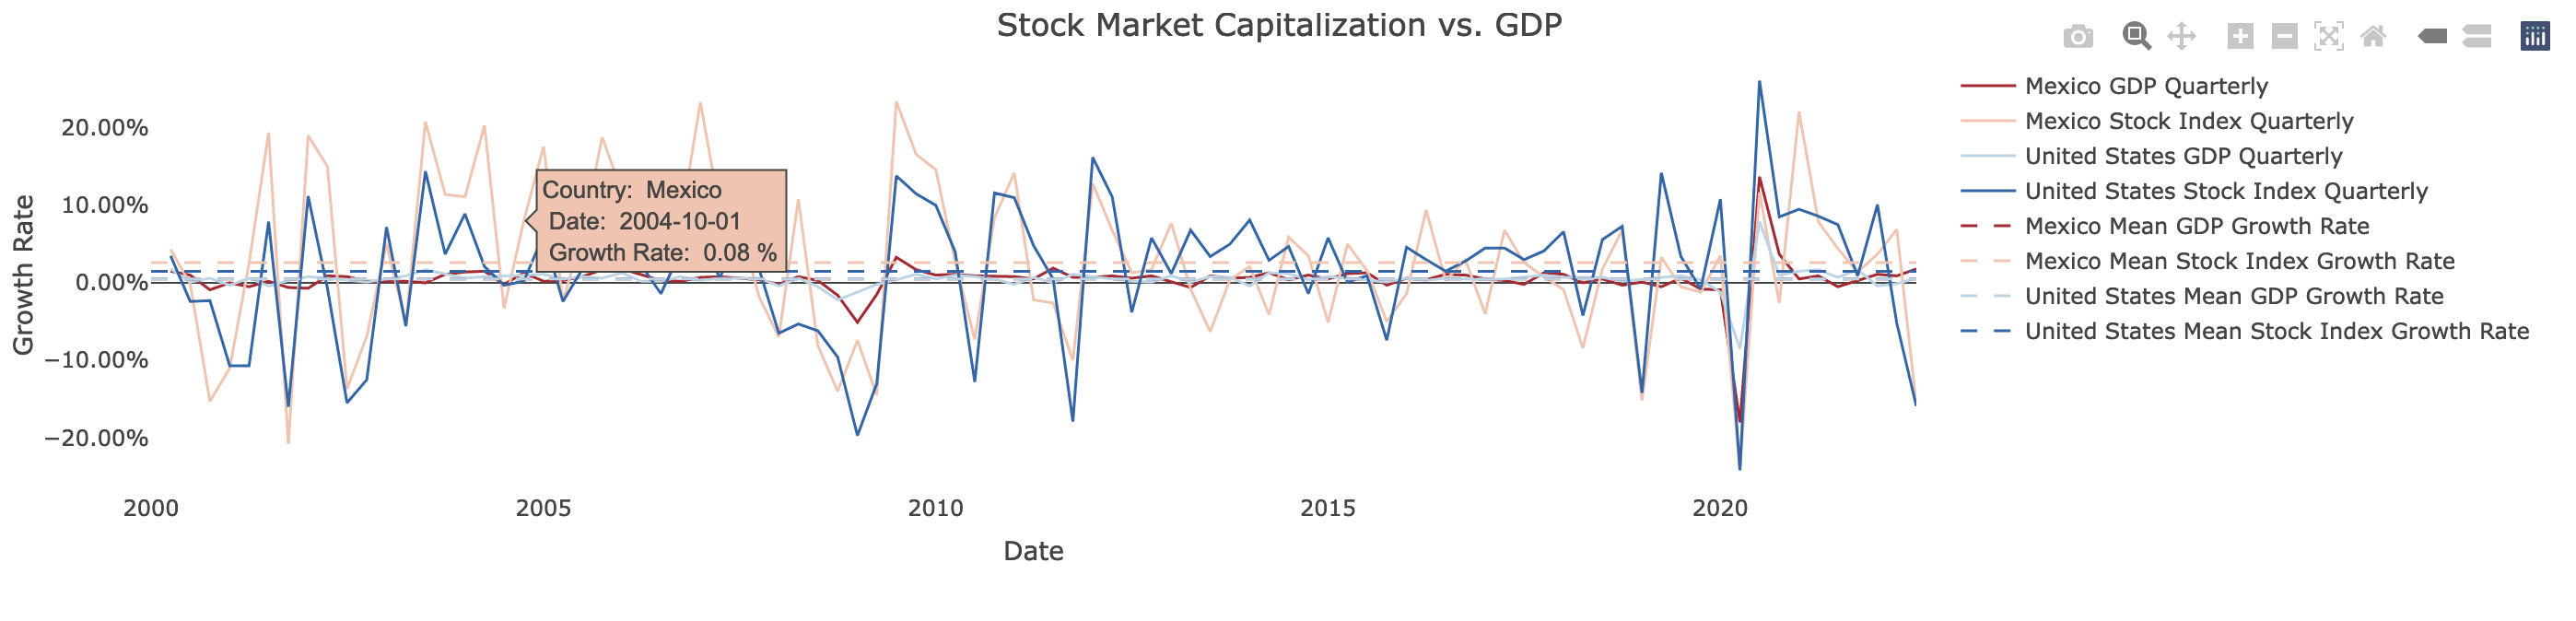
\includegraphics[width=15cm]{reports/figures/robustness_linechart.png}
    \caption{Shiny App Robustness Check: Interactive Line Chart, Box Plots and Histograms - \href{https://flurinaschneider.shinyapps.io/DTFF22/}{Interactive Shiny App}}
\label{robustness_linechart}
\end{figure}

\newpage
\section{Discussion}
In the United States, Indonesia and Mexico, the stock market is growing at a faster rate than the GDP for the examined time period (2000- 2022). The magnitude of the results differ depending on the development stage, the selected frequency and the date range. If we interpret the results based on the Buffet Indicator, there might be a indication for a bubble, according to the \cite{buffet}. \\


\indent In terms of limitations, we identify the following constraints for our research: We are not differentiating between industries. We only look at the aggregate market data and not individual companies , so we cannot say where (individual) deviations really come from. Also, since we use the SP500 and the SPY as a proxy for the US stock market, we introduce constraints there, since the index includes only a limited selection of companies. Additionally, we did not control for region-specific factors and also omitted a wide range of additional potentially relevant factors. 
In terms of further research, we recommend increasing the sample size, i.e. include more countries at different development stages in order to cross-reference. More data points should be collected, and the examined time span should be increased in order to provide more meaningful results as well as to give  historical context. We also suggest to control for additional factors (e.g. region-specific factors). 

\section{Conclusion}
In all three of the examined countries (United States, Indonesia and Mexico), the stock market is growing at a faster rate than GDP in the years 2000 to 2022. The magnitude of the results differs depending on development stage and the examined time intervals and date ranges. If we interpret the results according to the Buffet Indicator, our findings indicate the potential for a bubble. 

\newpage
\theendnotes

%\bibliography{citation/bibliography.bib}
%Alphavantage etc. (Input Luis)
%CFI
%Investopedia
%MSCI
%Worldbank


%Dmitry Kuvshinov, Kaspar Zimmermann,
%The big bang: Stock market capitalization in the long run,
%Journal of Financial Economics,
%Volume 145, Issue 2, Part B,
%2022,
%Pages 527-552,
%ISSN 0304-405X,
%https://doi.org/10.1016/j.jfineco.2021.09.008.
%https://www.sciencedirect.com/science/article/pii/S0304405X21003962


%Impact of the stock market capitalization and the banking spread in growth and development in Latin American: A panel data estimation with System GMM (article)
%Author
%Aali-Bujari,Ali and Venegas-Martínez,Francisco and Pérez-Lechuga,Gilberto
%Journal
%Contaduría y Administración
%Year
%2017
%Volume
%62
%Number
%5
%Pages
%1427--1441
%https://www.elsevier.es/es-revista-contaduria-administracion-87-articulo-impact-stock-market-capitalization-banking-S018610421730102X

%CitationMaría   A.   Prats   and   Beatriz   Sandoval   (2020).   Does   stock   marketcapitalization   cause   GDP?   A   causality   study   for   Central   and   Eastern   European   countries. Economics: The Open-Access, Open-Assessment E-Journal, 14 (2020-17): 1–29. http://dx.doi.org/10.5018/economics-ejournal.ja.2020-17
%https://www.degruyter.com/document/doi/10.5018/economics-ejournal.ja.2020-17/html

\printbibliography

%\bibliographystyle{apalike}

\appendix 

\section{Appendix}

\begin{figure}[H]
	\centering
	\includesvg[width=\textwidth]{figures/boxplots_growth_rates_all}
	\caption{Boxplots Indonesia and Mexico}
    \label{boxplots_indonesia_mexico}
\end{figure}

\begin{figure}[H]
	\centering
	\includesvg[width=\textwidth]{figures/histograms_growth_rates_all}
	\caption{Histograms Indonesia and Mexico}
    \label{histograms_indonesia_mexico}
\end{figure}

\begin{figure}[H]
	\centering
	\includesvg[width=\textwidth]{figures/regression_all_incomelevel}
	\caption{Regression of GDP vs. Stock Index: Indonesia and Mexico}
    \label{indonesia_mexico_regression}
\end{figure}

\begin{figure}[H]
	\centering
	\includesvg[width=\textwidth]{figures/growth_starting_at_100_all}
	\caption{Comparable growth rate of GDP vs Stock market: Indonesia and Mexico}
    \label{indonesia_mexico_growth_100}
\end{figure}







\end{document}